\chapter{Fundamentação Teórica}

\lipsum[1-2]

\begin{citacao}
\lipsum[1]\cite[p. ~34]{Huizinga2014}
\end{citacao}

\section{O que é Inteligência Artifical}


\lipsum[4-7]

\section{Processos Já automatizados com IA na área de TI}

\lipsum[8-9]

A figura \ref{fig:kings-landing} representa \emph{King's Landing}, cenário da série \emph{Game of Thromes} reproduzido no Minecraft:

\begin{figure}[h]
	\caption{\emph{The King's Landing} no Minecraft}
	\center
	\label{fig:kings-landing}
	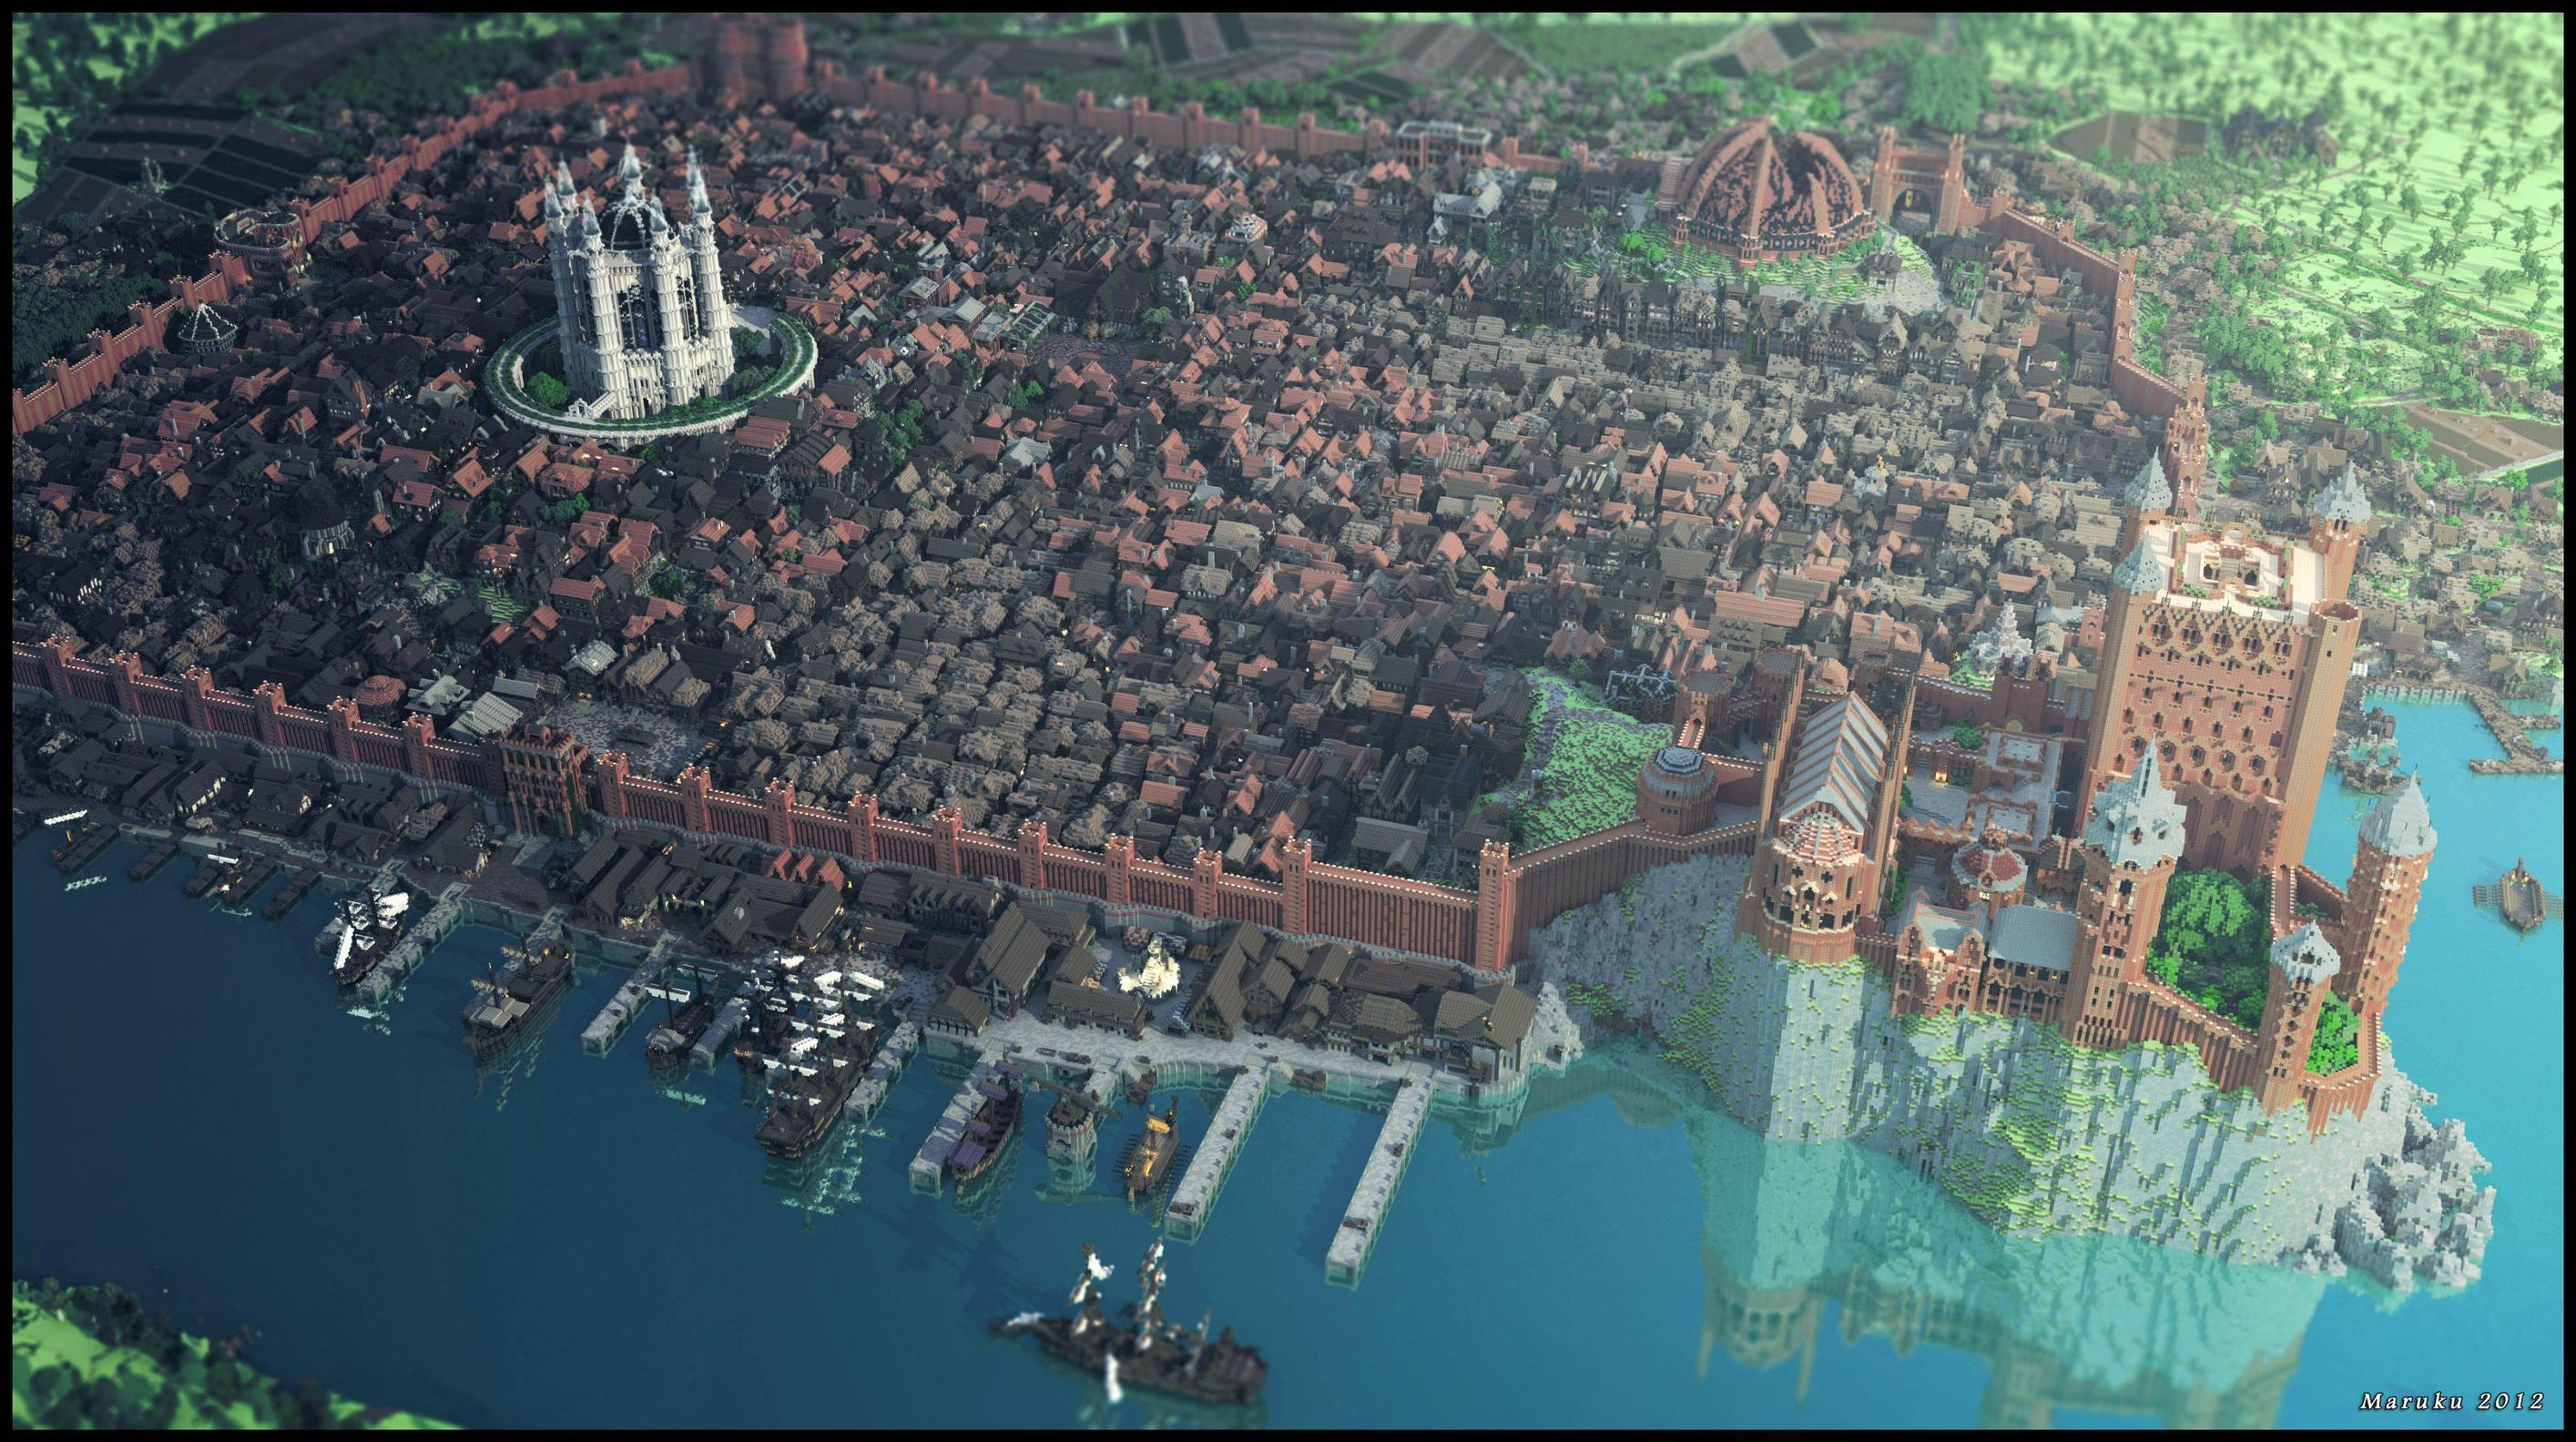
\includegraphics[scale=0.15]{fundamentacao/kings-landing.jpg}
	\fol{Imgur2013}
\end{figure}

\lipsum[10-12]


\section{O que é DB Autônomo}

\lipsum[1-2]


\section{Como funciona um Autônomo}

\lipsum[1-2]


\section{Quais os recursos que é possível automatizar do BD}

\lipsum[1-2]





\section{Qual o novo papel do DBA}

\lipsum[1-2]


\section{Ferramentas que existem e o que fazem}

\lipsum[1-20]

